\documentclass{../../sftex/sftex}

\usepackage{cancel, enumitem, tikz-qtree}

\title{Exemplo de poda $\alpha$-$\beta$ e função heurística para damas}
\author{Emmanuel Podestá Jr., Gustavo Zambonin}
\email{\{emmanuel.podesta,gustavo.zambonin\}@grad.ufsc.br}
\src{https://github.com/zambonin/ufsc-ine5430}
\uniclass{Inteligência Artificial}
\classcode{UFSC-INE5430}

\newcommand{\cc}[1]{\cancel{#1} \;}
\tikzset{every tree node/.style={align=center,anchor=north}}

\begin{document}

\maketitle

\begin{enumerate}[label= (\textbf{\arabic*})]

    \item Observações: locais marcados com um asterisco (*) são passíveis de
    poda caso existissem outros filhos. A árvore com raiz em um nodo
    ``cancelado'' (\cancel{exemplo}) foi podada pelo algoritmo.

    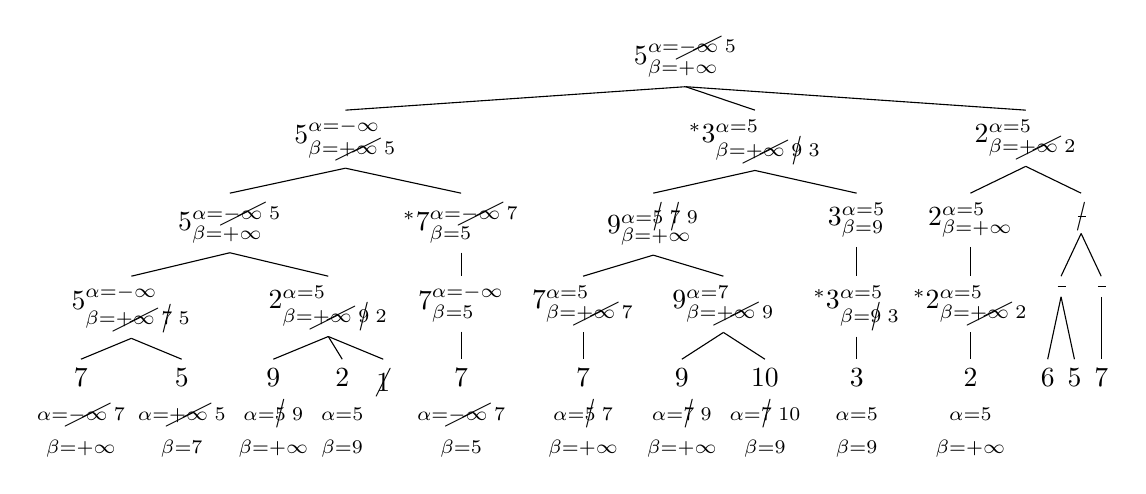
\begin{tikzpicture}[sibling distance=-2pt]

        \Tree
            [.$5_{\beta = +\infty}^{\alpha = \cc{-\infty} 5}$
                [.$5_{\beta = \cc{+\infty} 5}^{\alpha = -\infty}$
                    [.$5_{\beta = +\infty}^{\alpha = \cc{-\infty} 5}$
                        [.$5_{\beta = \cc{+\infty} \cc{7} 5}^{\alpha = -\infty}$
                            [ .{7 \\ $\scriptstyle\alpha = \cc{-\infty} 7$
                                    \\ $\scriptstyle\beta = +\infty$} ]
                            [ .{5 \\ $\scriptstyle\alpha = \cc{+\infty} 5$
                                    \\ $\scriptstyle\beta = 7$} ]
                        ]
                        [.$2_{\beta = \cc{+\infty} \cc{9} 2}^{\alpha = 5}$
                            [ .{9 \\ $\scriptstyle\alpha = \cc{5} 9$
                                    \\ $\scriptstyle\beta = +\infty$} ]
                            [ .{2 \\ $\scriptstyle\alpha = 5$
                                    \\ $\scriptstyle\beta = 9$} ]
                            [ .{\cancel{1}} ]
                        ]
                    ]
                    [.$^{*}7_{\beta = 5}^{\alpha = \cc{-\infty} 7}$
                        [.$7_{\beta = 5}^{\alpha = -\infty}$
                            [ .{7 \\ $\scriptstyle\alpha = \cc{-\infty}7$
                                    \\ $\scriptstyle\beta = 5$} ]
                        ]
                    ]
                ]
                [.$^{*}3_{\beta = \cc{+\infty} \cc{9} 3}^{\alpha = 5}$
                    [.$9_{\beta = +\infty}^{\alpha = \cc{5} \cc{7} 9}$
                        [.$7_{\beta = \cc{+\infty} 7}^{\alpha = 5}$
                            [ .{7 \\ $\scriptstyle\alpha = \cc{5} 7$
                                    \\ $\scriptstyle\beta = +\infty$} ]
                        ]
                        [.$9_{\beta = \cc{+\infty} 9}^{\alpha = 7}$
                            [ .{9 \\ $\scriptstyle\alpha = \cc{7} 9$
                                    \\ $\scriptstyle\beta = +\infty$} ]
                            [ .{10 \\ $\scriptstyle\alpha = \cc{7} 10$
                                    \\ $\scriptstyle\beta = 9$} ]
                        ]
                    ]
                    [.$3_{\beta = 9}^{\alpha = 5}$
                        [.$^{*}3_{\beta = \cc{9} 3}^{\alpha = 5}$
                            [ .{3 \\ $\scriptstyle\alpha = 5$
                                    \\ $\scriptstyle\beta = 9$} ]
                        ]
                    ]
                ]
                [.$2_{\beta = \cc{+\infty} 2}^{\alpha = 5}$
                    [.$2_{\beta = +\infty}^{\alpha = 5}$
                        [.$^{*}2_{\beta = \cc{+\infty} 2}^{\alpha = 5}$
                            [ .{2 \\ $\scriptstyle\alpha = 5$
                                    \\ $\scriptstyle\beta = +\infty$} ]
                        ]
                    ]
                    [.\cancel{\_}
                        [.\_
                            [ .{6} ]
                            [ .{5} ]
                        ]
                        [.\_
                            [ .{7} ]
                        ]
                    ]
                ]
            ]

    \end{tikzpicture}

    \item Considerando um jogo de damas usual e observando um modelo de grafo
    convencional, que mapeia estados do tabuleiro para nodos e jogadas válidas
    conectando-os como arestas, é possível observar que tal árvore resultante
    impossibilitará o uso de uma função utilidade apenas, por conta do seu
    vasto número de possibilidades para jogadas.

    Analisando as regras do jogo, alguns tópicos foram escolhidos de modo a
    diferenciar um tabuleiro que representa uma boa jogada. Estes podem ser
    utilizados para ambos os tipos de funções.

    \begin{itemize}

        \item É necessário normalizar o valor do tabuleiro em relação ao
        jogador humano, então pode-se decrementar da pontuação deste o valor
        obtido pela análise das peças do jogador computacional.

        \item O número de ``damas'' do jogador deve influenciar mais no valor
        final do tabuleiro do que peças normais, visto que é mais difícil
        obtê-las e sua capacidade de movimentação e ataque são melhoradas.

        \item O número de peças no tabuleiro é um fator a ser considerado,
        visto que é muito mais difícil vencer um jogo se suas peças estão
        cercadas por outras de cor diferente.

        \item As possibilidades de ataque de peças normais e ``damas'' devem
        ser consideradas, de modo que o algoritmo deve verificar se existem
        movimentos que possam remover uma ou mais peças do adversário; porém,
        tais verificações serão mais custosas em virtude do incremento da
        procura em profundidade para considerar ataques duplos ou triplos.

    \end{itemize}

    Note que tais análises são extremamente ingênuas; para produzir um jogador
    computacional hábil, recursos como a pré-computação de valores para estados
    de tabuleiros específicos, na forma de bancos de dados; grandes listagens
    de movimentos de abertura, para maximizar a chance de boas jogadas desde o
    começo; e otimizações como tabelas de transposição\footnote{tabelas que
    guardam estados de tabuleiro que são iguais e alcançáveis por um grande
    número de jogadas diferentes; ou seja, caso uma jogada já tenha sido
    descartada e um tabuleiro similar aparece novamente, uma consulta nesta
    tabela pode acelerar a procura de possibilidades no algoritmo, descartando
    este tabuleiro.} podem ser inseridos no algoritmo para que seu conhecimento
    seja aumentado. Todos estes exemplos foram aplicados no jogador
    \textit{Chinook}~\cite{Schaeffer1989}.

\end{enumerate}

\bibliography{ine5430_t1}
\bibliographystyle{plain}

\end{document}
